\documentclass[a4paper, 10pt, twoside, notitlepage]{article}
% idioma
\usepackage[spanish]{babel}
\usepackage[utf8x]{inputenc}
% graficos
\usepackage[pdftex]{graphicx}

\usepackage{wrapfig}
\usepackage{amsmath}
\usepackage{tikz}
\usepackage{mathdots}
\usepackage{yhmath}
\usepackage{cancel}
\usepackage{color}
\usepackage{siunitx}
\usepackage{array}
\usepackage{multirow}
\usepackage{amssymb}
\usepackage{gensymb}
\usepackage{tabularx}
\usepackage{booktabs}
\usetikzlibrary{fadings}
\usepackage{xfrac}

%\usepackage{listings}
%\lstset{language=C,basicstyle=\small}

%\usepackage{epic,eepic}
% estilo
\usepackage[footnotesize]{caption}
\usepackage[outer=2cm,inner=4cm,top=2cm,bottom=2cm]{geometry}
\usepackage{fancyhdr}

\usepackage{color,hyperref}
\usepackage{enumerate}

\definecolor{black}{rgb}{0.0,0.0,0.0}
\definecolor{darkblue}{rgb}{0.0,0.0,0.3}

\hypersetup{colorlinks,breaklinks,
            linkcolor=black,urlcolor=darkblue,
            anchorcolor=darkblue,citecolor=darkblue}
            
\usepackage{blindtext}
\usepackage{listings}
% matematica
\usepackage{amsmath} 
\usepackage{amsfonts} 
\usepackage{amssymb}
\usepackage{enumitem}



 \title{U.B.A. - Facultad de Ingeniería\\\vspace{0.25cm} 66.20 Organización de Computadoras\\Guía de ejercicios}
  \author{Práctica jueves}
 \date{1° Cuatrimestre 2019}


\definecolor{mymauve}{rgb}{0.58,0,0.82}
\definecolor{mygreen}{rgb}{0,0.6,0}

\date{}

\begin{document}

\lstset{%
  basicstyle=\small\ttfamily,
  breaklines=true,
  tabsize=2,
  language=C,
  extendedchars=true
}

\lstdefinestyle{6620C}{
  identifierstyle=\color{blue},
  commentstyle=\color{mygreen},
  keywordstyle=\bfseries\color{mymauve},
  frame=single,
  breaklines=true
%  stringstyle=\color{purple}
}


\maketitle
\thispagestyle{empty}   % quita el número en la primer página

%\newpage
%\begin{abstract}

%\end{abstract}

%\tableofcontents
% 
 \newpage
% 

\pagestyle{fancy}
\fancyhead{}
\fancyfoot{}
\renewcommand{\sectionmark}[1]{\markright{\thesection\ #1}}
\renewcommand{\headrulewidth}{0.4pt}
%\renewcommand{\footrulewidth}{0.4pt}
\fancyhead[LE]{\nouppercase \rightmark}
\fancyhead[RE, LO]{\bf \thepage}
\fancyhead[RO]{\nouppercase \rightmark}
\fancyfoot[C]{ }
\maketitle
%genera el indice - compilar dos veces
\setcounter{page}{1}
% \tableofcontents
% \newpage

\parskip 7.2pt

\section{Principios fundamentales}
\subsection{}
Demostrar que 

						 $$ SU = \frac {1} {(1-f) + \frac {f}{SU_l}} $$


Donde $f$ es la fracción de tiempo a mejorar, y $SU_l$ es la mejora local.

\subsection{}

Un procesador de 300 Mhz ejecuta un programa que presenta los siguientes tipos de instrucciones:

\begin{table}[h!]
\begin{tabular}{|l|c|c|}
\hline
 Tipo de instrucción & Frecuencia (\%)  &  Ciclos  \\ \hline
 Aritmético-Lógica & 40  &  1  \\ \hline
 Carga & 20 & 1 \\ \hline
 Almacenamiento & 10  & 2  \\ \hline
 Saltos & 20  & 3 \\ \hline
 Punto Flotante & 10 & 5  \\ \hline
\end{tabular}
\end{table}

\begin{enumerate}[label=\alph*)]
 \item Calcular las tasas de CPI y MIPS, para el programa completo.
 \item Suponga que una optimización elimina un 30 \% de las instrucciones aritmético-lógicas (o sea, 12 \% del total de instrucciones A-L), 30 \% de instrucciones load y 20 \% de punto flotante. ¿Cuál es el speedup alcanzado?
 \item Recalcular las tasas de CPI y MIPS para el programa completo. Explicar las diferencias respecto al punto (a).
\end{enumerate}

\subsection{}
Se proponen 3 mejoras para una nueva arquitectura con los siguientes Speedups:
\begin{itemize}
\item Speedup1 = 30
\item Speedup2 = 20
\item Speedup3 = 10
\end{itemize}

Sólo una mejora es aplicable en cada momento (no se pueden solapar).

\begin{enumerate}[label=\alph*)]
 \item Si las mejoras 1 y 2 se pueden usar un 30 \% del tiempo, ¿qué fracción del tiempo se debe usar la mejora 3 para lograr un speedup global de 10?
 \item Asumir que la distribución del uso de las mejoras es del 30 \%, 30 \% y 20 para las mejoras 1, 2 y 3 respectivamente. Asumir que las 3 mejoras están en uso. ¿Qué fracción del tiempo mejorado no tiene una mejora en uso?
 \item Asumir que para un benchmark la fracción del uso de las mejoras es del 15 \% para 1 y 2 y del 70 \% para la mejora 3. Se quiere maximizar la performance. Si sólo una mejora puede ser aplicada, ¿cuál debería ser elegida? Si 2 mejoras pueden ser aplicadas, ¿cuales deberían ser elegidas?
\end{enumerate}

\subsection{}
Se dispone de un benchmark que contiene $195,578$ instrucciones de punto flotante.
	
Dicho Benchmark fue ejecutado en un procesador embebido luego de haber sido compilado con las optimizaciones activadas. El procesador embebido está basado en un procesador RISC que incluye unidades de punto flotante, pero el procesador embebido no dispone de ellas por distintas razones. El compilador permite calcular las operaciones de punto flotante mediante unidades punto flotante o mediante rutinas de software, dependiendo en las opciones utilizadas.
	
El benchmark se ejecutó en $1,08$ segundos en el procesador RISC, mientras que tomó $13.6$ segundos en la versión embebida. Asumir que el CPI del procesador RISC es $10$, mientras que el CPI del procesador embebido es $6$.
	
\begin{enumerate}[label=\alph*)]
\item Para ambos procesadores, ¿cuántas instrucciones fueron ejecutadas?
\item Para ambos procesadores, ¿cuál es el valor de la tasa de MIPS?
\item En promedio, ¿cuántas instrucciones enteras son necesarias para ejecutar una operación de punto flotante en software?
\end{enumerate}
	
Responder considerando que el benchmark puede estar conformado por 
	
\begin{itemize}
    \item Un $100\%$ de instrucciones de punto flotante.
    \item Instrucciones de punto flotante y enteras.
\end{itemize}

\subsection{[1.2 $3^{ed}$ CAAQA]}
Se considera realizar una mejora a una máquina agregando hardware vectorial. Cuando un cálculo de modo vectorial se ejecuta en este hardware, este se realiza 10 veces más rápido que en modo de ejecución normal. Llamamos al porcentaje de tiempo que se puede utilizar este modo vectorial como porcentaje de vectorización.

\begin{enumerate}
 \item Realizar un gráfico que represente el speedup en función del como porcentaje de vectorización. Nombrar al \textit{eje y} como Speedup Global y al \textit{eje x} como Porcentaje de Vectorización.
 
 \item ¿Qué porcentaje de vectorización en necesaria para alcanzar un speedup global de 2?
 
 \item ¿Qué porcentaje de tiempo se emplea en modo vectorización cuando se alcanza un speedup global de 2?
 
 \item ¿Qué porcentaje de vectorización es necesaria para alcanzar la mitad del máximo speedup posible al usar el modo de vectorización?
 
 \item Ahora suponga que se realizó una medición y se determinó que el porcentaje de vectorización para ciertos programas es del 70\%. El grupo de diseño de hardware dice que pueden duplicar el speedup del hardware de vectorización pero con una inversión significante en lo que respecta. Entonces nos preguntamos si el equipo de compiladores podrían incrementar el uso del modo vectorizado (relativo al uso actual) para lograr la misma performance obtenida al aumentar al doble el speedup por hardware. ¿Qué inversión recomendaría?  
\end{enumerate}


\subsection{[1.3 $3^{ed}$ CAAQA]}
Se realiza una mejora a una computadora a un dado modo de ejecución por un factor de 10. Esta mejora es utilizada el 50\% del tiempo, medido como un porcentaje del tiempo de ejecución cuando la mejora está siendo utilizada. Recordar que no se puede aplicar directamente este 50\% en la Ley de Amdahl para para calcular el speedup.

\begin{enumerate}
 \item ¿Cuál es el speedup global que se alcanza con esta mejora?
 \item ¿Qué porcentaje del tiempo original es empleada esta mejora?
\end{enumerate}


\subsection{[1.6 $3^{ed}$ CAAQA]}
Un benchmark muy conocido para enteros es Dhrystone. La computadora A realiza D A ejecuciones del benchmark por segundo y realiza millones de instrucciones por segundo (MIPS A). En la computadora B se ejecuta el mismo benchmark obteniendo sus propias métricas.

\begin{enumerate}
 \item ¿Cuál es el problema en calcular la tasa de MIPS de la computadora B como $MIPS_B = MIPS_A \times (D_B / D_A )$?
\end{enumerate}



\subsection{[1.17 $3^{ed}$ CAAQA]}
Una empresa tiene un benchmark que es considerado representativo para sus aplicaciones típicas. Se está considerando un procesador embebido para realizar las tareas pero no cuenta con una unidad de punto flotante y se deben emular por una secuencia de instrucciones de enteros. Este procesador tiene una tasa de 120 MIPS en el benchmark.

Un vendedor ofrece un coprocesador para mejorar la performance. Este coprocesador ejecuta cada instrucción de punto flotante por hardware. Cuando se combina el procesador y el coprocesador resulta una tasa de MIPS de 80 en el mismo benchmark.

Sea:

\begin{itemize}
 \item I: Número de instrucciones de enteros ejecutadas en el benchmark.
 \item F: Número de instrucciones de punto flotante ejecutadas en el benchmark.
 \item Y: Número de instrucciones de entero para emular las instrucciones de punto flotante.
 \item W: Tiempo de ejecución del benchmark en el procesador solo.
 \item B: Tiempo de ejecución del benchmark en la combinación procesador/coprocesador.
\end{itemize}

\begin{enumerate}
 \item Escribir una expresión para calcular la tasa de MIPS en cada configuración utilizando los símbolos anteriores.
 \item Para la configuración sin coprocesador, se obtuvo $F = 8 \times 10^6$, $Y = 50$ y $W = 4$ segundos. Determinar I.
 \item ¿Cuál es el valor de B?
 \item ¿Cuál es la tasa de MFLOPS para el sistema con coprocesador?
 \item Un colega quiere comprar el coprocesador a pesar que tiene una tasa de MIPS inferior cuando se lo utiliza en comparación con el procesador sólo. ¿Tiene razón? Justificar la respuesta.
\end{enumerate}



\newpage
\chapter{Arquitectura de programación}
El término arquitectura del conjunto de instrucciones (instruction set architecture) (ISA) se refiere al conjunto de instrucciones visibles al programador. Funciona como la frontera entre el software y el hardware.


\section{Modelo de pila}
Los operandos en una arquitectura de stack están implícitamente en el tope del stack y el hardware debe evaluar la expresión en un solo orden y cargar un operando múltiples veces.


\section{Modelo de acumulador}
En una arquitectura de acumulador un operando está implícito en el acumulador.


\section{Modelo de registros de propósito general}
En la arquitectura de registros de propósito general se tienen únicamente operandos explícitos, ya sea que estén ubicados en registros o en memoria.

Los operandos explícitos podrían ser accedidos directamente de memoria o necesitar ser cargados de memoria a un registro temporal dependiendo de la arquitectura y de la instrucción específica.


\section{Modelo de carga y almacenamiento}

En este tipo de arquitectura, la memoria solo puede ser accedida a través de instrucciones de carga y almacenamiento (load/store). 

\subsection{Conjunto de instrucciones RISC}

Las arquitecturas RISC se caracterizan por tener ciertas propiedades que simplifican su implementación.

\begin{itemize}
\item Todas las operaciones de datos aplican a datos en registros y típicamente modifican todo el registro (32 o 64 bits por registro).
\item Las únicas operaciones que afectan a la memoria son de carga y almacenamiento (load y stores) que mueven datos de la memoria a un registro o viceversa. Estas operaciones pueden mover datos menores que la capacidad de un registro (por ejemplo 16 bits).
\item El número de formatos de instrucciones son pocos con todas las instrucciones del mismo tamaño.
\end{itemize}

Como otras arquitecturas RISC, el conjunto de instrucciones de MIPS tiene 32 registros, aunque el registro 0 siempre tiene el valor 0. 

Hay tres tipos de instrucciones:

\begin{enumerate}
\item Instrucciones ALU. Estas instrucciones toman dos registros o bien un registro y un inmediato de signo extendido, realiza la operación y almacena el resultado en otro registro.

\item Instrucciones Load / Store. Estas instrucciones toman un registro base, y un inmediato como offset. La suma resultante del contenido del registro y el offset da la dirección efectiva y es usada para direccionar la memoria. En el caso de un store, el segundo registro opera como fuente del dato que se almacena en memoria.

\item Branches  y  jumps. Branches son transferencias condicionales del flujo de control. La forma de especificar la condición del branch, MIPS compara entre un par de registros o entre un registro y cero.

El destino del branch se obtiene sumando un offset con extensión de signo (16 bits) al valor actual del PC.
\end{enumerate}

\subsection{Modos de direccionamiento}
\subsection{Formato de instrucciones}

\newpage
\section{Jerarquia de memoria}

\subsection{}
Sea una computadora MIPS32, con un CPI ex de 2 y una frecuencia de clock de 1GHz, con una
memoria que tiene 100ns de latencia y 200MHz de ancho de banda, en la que ejecutamos el siguiente
programa:

\begin{verbatim}
$L9:
    addu    $v0,$v0,$a1
    sw      $v1,0($v0)
    addu    $v1,$v1,1
    sltu    $v0,$v1,$a0
    sll     $v0,$v1,2
    bne     $v0,$zero,$L9
\end{verbatim}

Si el registro \texttt{\$a0} contiene el valor 200, el registro a1 contiene el valor \texttt{0xcafebeb0}, y el programa está almacenado a partir de \texttt{0x0000f000}

\begin{enumerate}[label=\alph*)]
 \item ¿Cuánto tarda en ejecutarse el programa?
 \item ¿Qué proporción de este tiempo ocupan los ciclos de stall?
 \item Si agregamos un caché split LRU de mapeo directo y bloques de 16 bytes, de 32KB de tamaño
tanto para L1I como para L1D, con un $T_{hit}$ que no retrasa a la CPU, ¿cuánto tardaría en
ejecutarse el programa si L1D es WB/WA?
 \item ¿Cuáles serían los conjuntos ocupados en las dos caches?
 \item ¿Cuánto tardaría si L1D es $WT/¬WA$?
\end{enumerate}

\subsection{}
Se dispone de una computadora MIPS32 con 32MB de memoria, sin niveles de cache e inicialmente sin soporte para memoria virtual. La memoria tiene un tiempo de acceso promedio de 100 ciclos. En esta computadora se ejecuta la siguiente función:

\begin{verbatim}
void mat_transpose(int **mat, int **mat_trans, size_t n) {
    register unsigned int i, j;
    for (i = 0; i < n; i++) {
        for (j = 0; j <= i; j++) {
            mat_trans[j][i] = mat[i][j];
            mat_trans[i][j] = mat[j][i];

        }
    }
}
\end{verbatim}

La función \texttt{mat\_transpose()} recibe una matriz de enteros como primer argumento, y escribe
en la dirección indicada por \texttt{mat\_trans} la matriz transpuesta. Las matrices son cuadradas, de $n
\times n$ enteros.

\begin{enumerate}[label=\alph*)]
 \item Si la computadora no dispone de soporte para memoria virtual, ¿cuál es el máximo tamaño
que puede tener cada matriz?
 \item A partir de este punto se decide brindar soporte para memoria virtual. En un principio, el
único parámetro definido es que el tamaño de página es de 4 KB. Si se utilizan matrices cuadradas de $32 \times 32$, indicar cuanta memoria se necesita para soportar el sistema de traducción
para cada caso, siempre considerando que cada entrada de la tabla ocupa 4 bytes.
 
\begin{enumerate}[label=\roman*)]
 \item Si se utiliza una tabla de páginas lineal. 
 \item Si se utiliza una tabla de páginas jerárquica de dos niveles, de manera que cada tabla ocupa una página de memoria física.
 \item Si se utiliza una tabla de páginas invertida (sin HAT).
\end{enumerate}

 \item Finalmente, se decide utilizar una tabla jerárquica de dos niveles. Indicar el tiempo promedio
de acceso a los datos de las matrices, considerando únicamente la ejecución de la función
\texttt{mat\_transpose}.
 \item Ídem, considerando que se agrega un TLB completamente asociativo de 64 entradas.
\end{enumerate}

\subsection{}
Se brinda a continuación una serie de referencias a memoria, dadas como direcciones de palabras: 2, 3, 11, 16, 21, 13, 64, 48, 19, 11, 3, 22, 4, 27, 6 y 11. Suponer una memoria caché de correspondencia directa con 16 bloques de una palabra inicialmente vacíos. Rotular cada referencia de la lista como ``acierto''(\textit{hit}) o ``desacierto'' (\textit{miss}) y mostrar el contenido final de la caché.

\subsection{}
Usando la serie de referencias dadas en el ejercicio anterior, mostrar los aciertos y desaciertos y el contenido final de la memoria caché para una organización de correspondencia directa con bloques de cuatro palabras y un tamaño total de 16 palabras.

\subsection{}
Suponer que se tienen dos computadoras idénticas A y B, salvo por su organización de memoria caché. Se pide la escritura de dos códigos de manera tal que se cumpla que el primer código se ejecute mucho más rápido en la máquina A que en la B, y que el segundo código se ejecute mucho más rápido en la máquina B que en la A.

Datos:

\begin{itemize}
 \item Caches unificadas.
 \item El tiempo de escritura de una palabra de 32 bits en memoria principal es igual a 5 tiempos de acierto en memoria caché.
 \item Penalidad de desacierto = 10 tiempos de acierto. 
 \item Caché A: 128 conjuntos, dos elementos por conjunto, bloque de 32 bytes, \textit{write through} y \textit{no-write allocate}.
 \item Caché B: 256 conjuntos, un elemento por conjunto, bloque de 32 bytes, \textit{write back} y \textit{write allocate}.
\end{itemize}

\subsection{}
Dado el siguiente pseudocódigo:

\small
\begin{verbatim}
    int array[10000,100000];

    para cada elemento array[i][j]
        array[i][j] = array[i][j]*2;
\end{verbatim}
\normalsize

\begin{enumerate}
 \item Escribir dos programas en C que implementen este algoritmo: uno debe acceder los elementos del array recorriéndolo por filas (\textit{row-major order}) y el otro debe accederlos recorriéndolo por columnas (\textit{column-major order}).
 \item Compare los tiempos de ejecución de los dos programas.
 \item ¿Cómo explica los resultados obtenidos en base al impacto que el código ha producido en la jerarquía de memoria? 
\end{enumerate}

 
\subsection{}
Suponer dos memorias caches: C1 es una organización de correspondencia directa con 16 bloques de una palabra y C2 es una organización de correspondencia directa con bloques de cuatro palabras y un tamaño total de 16 palabras. Suponer una penalidad de desacierto para C1 de 8 ciclos de reloj de \textit{bus} y una penalidad de desacierto para C2 de 11 ciclos de reloj de \textit{bus}. Suponiendo que las caches están inicialmente vacías, encontrar una secuencia de referencias para la cual C2 tenga una tasa de desaciertos (\textit{miss rate}) más baja pero pase más ciclos de reloj en desaciertos de caché que C1. Usar direcciones de palabras.

\subsection{}
Para una computadora con CPU MIPS R2000 y memoria caché de 16-KB con asociatividad de grado 4 y línea de 16 bytes:

\begin{enumerate}
 \item Calcular el número de bits de \textit{tag}, \textit{índice} y \textit{offset}.
 \item Dibujar un esquema detallado de la memoria caché (numerar los conjuntos desde 0 en adelante).
 \item Dar la dirección (en hexadecimal) correspondiente a cada uno de los siguientes datos y ubicarlos en el esquema del ítem b:

\begin{enumerate}
 \item A y B son datos de un mismo bloque de memoria que mapean en el conjunto número 7.
 \item C y D son datos de distintos bloques de memoria que mapean en el conjunto número 255.
 \item E y F son datos que pertenecen a los bloques de memoria principal siguientes a C y D, respectivamente.
 \item G es un dato separado en 1-MB de distancia respecto a B. 
\end{enumerate}
\end{enumerate}

\subsection{}
Dar una secuencia de 5 direcciones de memoria distintas generadas por una CPU MIPS con memoria caché, de manera tal que se cumpla con lo siguiente:

\begin{itemize}
 \item La segunda dirección es acierto.
 \item La tercera mapea en un conjunto distinto al correspondiente a la primera.
 \item La quinta es desacierto.
\end{itemize}

Las direcciones se deben dar en hexadecimal. La memoria caché es de 8-KB, asociativa de grado 2 y bloque de 16 bytes. No se pueden hacer hipótesis acerca del contenido previo de la caché. Justificar su respuesta.

\subsection{}
Para el siguiente código:

\small
\begin{verbatim}
        add $t2, $0, $0
loop:   sll $t1, $t2, 2
        sw $t2, array($t1)
        addi $t2, $t2, 1
        slti $t3, $t2, 12
        bgtz $t3, loop
        ori $v0, $0, 10
        syscall

.data
.align 5
array:  .word 0, 1, 2, 3, 4, 5, ...
\end{verbatim}
\normalsize

\begin{enumerate}
 \item Calcular el CPI promedio.
 \item Calcular el promedio de accesos a memoria por instrucción.
 \item Calcular la tasa de desaciertos.
\end{enumerate}

Datos: caché de 8-KB, de 2 vías asociativa por conjunto, unificada, con bloque de 32 bytes y política de reemplazo LRU. Aclare las hipótesis que utilice.

\subsection{}
Para una computadora con CPU MIPS R2000 y memoria caché de 512 bytes con asociatividad de grado 2 y línea de 16 bytes.

\begin{enumerate}
 \item Calcular el número de bits de \textit{tag}, \textit{índice} y \textit{offset}.
 \item Dibujar un esquema detallado y completo de la memoria caché (área de datos y \textit{tags}). Numerar los conjuntos desde 0 en adelante.
 \item Ubicar en el dibujo a cada uno de los siguientes datos (bytes) dados por su dirección, y dar y ubicar en el área de \textit{tags}, a los \textit{tags} correspondientes.

\begin{center}
\begin{tabular}{cc}
Dato        &   Dirección       \\
\tt A	    &   \tt 0xffffff00  \\
\tt B	    &   \tt 0xffffff04  \\
\tt C	    &   \tt 0xcccccc08  \\
\tt D	    &   \tt 0xffffff1a  \\
\tt E	    &   \tt 0xffffff70  \\
\tt F	    &   \tt 0xffffffff  \\
\end{tabular}
\end{center}
\end{enumerate}

Justifique todas sus respuestas y muestre sus cálculos.


\subsection{}
Supongamos tener 3 computadoras con las siguientes configuraciones de memoria caché: (C1) DM, (C2) 2WSA y (C3) FA (i.e completamente asociativo). En todos los casos, se trata de sistemas de alojamiento unificados, en donde la capacidad es de 8 líneas de 32 bit cada una, con reemplazo LRU. 

\begin{center}
	\begin{small}
	\begin{verbatim}
   # Benchmark B0                 # Benchmark B1
      li    t1, 100                  li t1, 100
loop: lw    t2, 1024(zero)     loop: lw t2, 1028(zero)
      subu  t1, t1, 1                subu t1, t1, 1
      bnez  t1, loop                 bnez t1, loop
   \end{verbatim}
  \end{small}

  \begin{small}
  \begin{verbatim}
	 # Benchmark B2                 # Benchmark B3             # Benchmark B4
      li    t1, 100                  li t1, 100                 li t1, 100
loop: lw    t2, 1028(zero)     loop: lw t2, 1028(zero)    loop: lw t2, 1028(zero)
      lw    t2, 1032(zero)           lw t2, 1032(zero)          lw t2, 1032(zero)
      subu  t1, t1, 1                lw t2, 1036(zero)          lw t2, 1036(zero)
      bnez  t1, loop                 subu t1, t1, 1             lw t2, 1040(zero)
                                     bnez t1, loop              subu t1, t1, 1
                                                                bnez t1, loop
	\end{verbatim}
	\end{small}
\end{center}

Suponiendo que todos los \emph{benchmarks} comienzan con la primera	instrucción en la dirección de memoria nula.

\begin{enumerate}
 \item	?`Cuál es el \emph{benchmark} con mejor desempeño en el caché C1?
 \item	?`Cuáles de 0\% 25\% 50\% 75\% 100\% representa mejor la tasa de acierto para B1+C1?
 \item	?`Qué caché tiene mejor tasa de acierto con B3?
 \item	?`Cuál caché, logra una tasa de acierto nula con B4? Elegir uno de C1, C2, C3, o ninguno.
\end{enumerate}


\subsection{}
Para el siguiente sistema:

\begin{itemize}
 \item Microprocesador: 1Ghz
 \item CPI (sin accesos a memoria): 0,7
 \item Del total de instrucciones, 20\% son lecturas, 5\% son escrituras
 \item Cache L1 Instrucciones: 
 \begin{itemize}
  \item Direct Mapped
  \item 32KB de Tamaño
  \item 32 bytes por bloque
  \item Write Back.
  \item 2\% de tasa de miss. Tiempo de hit despreciable.
 \end{itemize}
  \item Cache L1 Datos:
  \begin{itemize}
   \item Direct Mapped
   \item 32KB de Tamaño
   \item 32 bytes por bloque
   \item Write Through
   \item 5\% de tasa de miss. Tiempo de hit despreciable.
  \end{itemize}
  \item Cache L2:
  \begin{itemize}
   \item 512Kb de Tamaño
   \item 32 bytes por bloque
   \item Write Back
   \item 15ns de tiempo de hit
   \item 80\% de tasa de hit
   \item 50\% de bloques en estado dirty
  \end{itemize}
 \item Memoria Principal:
 \begin{itemize}
  \item 40ns de latencia
  \item Ancho de bus 64 bits
  \item Clock de memoria principal 5ns
  \item 200Mhz de Ancho de banda
 \end{itemize}
\end{itemize}

\begin{itemize}
 \item ¿Cuál es el tiempo promedio de acceso a memoria para leer una instrucción?
 \item ¿Cuál es el tiempo promedio de acceso a memoria para leer un dato?
 \item ¿Cuál es el tiempo promedio de acceso a memoria para escribir un dato?
 \item ¿Cuál es el CPI promedio, teniendo en cuenta los accesos a memoria?
\end{itemize}
	
\subsection{}  
Para este problema, asumir que se tiene un procesador con un caché	conectado a memoria principal vía un bus. Un caché hit toma 1 ciclo. Luego de un miss, un bloque se transfiere desde memoria principal sobre el bus. El fetch del bloque no se inicia hasta que comienza el ciclo siguiente al del miss.

Una transacción en el bus consiste de un ciclo para enviar la dirección de memoria, 4 ciclos de idle time para el acceso a memoria principal, y luego un ciclo para transferir cada word del bloque desde memoria principal hacia el caché.

Asumir que el procesador continúa la ejecución sólo después de que el último word del bloque ha sido transferido.

En otras palabras, si el tamaño de bloque es B words (32 bits/word), un caché miss costará 1+1+4+B ciclos.

El cuadro \ref{tbl:B_vs_m} muestra el miss rate promedio del caché para un caché de 1MB para varios tamaños de bloques.

\begin{table}[h]
\begin{center}
\begin{tabular}{c|c}
B [words] & m [\%]  \\\hline
1  & 3.4  \\
4  & 1.1  \\
8  & 0.43 \\
16 & 0.28 \\
32 & 0.19 \\
\end{tabular}
\caption{Tamaño de bloque (B) vs. Miss rate (m)}
\label{tbl:B_vs_m}
\end{center}
\end{table}

\begin{enumerate}
\item Escribir una expresión para el tiempo promedio de acceso a memoria, en términos de $m$ y $B$.
\item ¿Qué tamaño de bloque otorga el mejor tiempo promedio de acceso a memoria?
\item Si la contención por el acceso al bus agrega 3 ciclos al tiempo de acceso a memoria principal, ¿qué tamaño de bloque otorga el mejor tiempo promedio de acceso a memoria?
\item Si el ancho del bus se cuadruplica a 128 bits, reduciendo el tiempo que toma la transferencia del bloque (dentro de la transacción en el bus) a un 25\% del valor original, ¿cuál es el tamaño de bloque óptimo?

Asumir que como mínimo se requiere 1 ciclo para la transferencia, y no incluir los ciclos de contención mencionados en el ítem anterior.
\end{enumerate}

\subsection{}
Para cada uno de los siguientes puntos, elegir la respuesta correcta justificando su elección (la respuesta siempre se toma como errónea si no está debidamente justificada)

\begin{enumerate}
\item	Si el acceso a caché requiere un ciclo de reloj y cada caché
		miss produce un \emph{stall} de 5 ciclos adicionales, ¿cuál de
		los siguientes \emph{caché hit rates} se acerca más a lograr un
		acceso promedio a memoria de 2 ciclos?

		\begin{enumerate}
		\item	$75\%$
		\item	$80\%$
		\item	$83\%$
		\item	$86\%$
		\item	$98\%$
		\end{enumerate}
\item	LRU es una estrategia de reemplazo en caches efectiva
		principalmente debido a que los programas \ldots

		\begin{enumerate}
		\item	\ldots exhiben localidad de referencias a memoria
		\item	\ldots usualmente trabajan en regiones de memoria
			pequeñas
		\item	\ldots leen datos más frecuentemente de lo que los
			escriben
		\end{enumerate}
\item	Si incrementar el tamaño de bloque de un caché mejora su
		performance, esto se debe principalmente a que los programas 
		\ldots

		\begin{enumerate}
		\item	\ldots exhiben localidad de referencias a memoria
		\item	\ldots usualmente trabajan en regiones de memoria pequeñas
		\item	\ldots leen datos más frecuentemente de lo que los escriben
		\end{enumerate}

\item	Dado el siguiente programa:
		\begin{small}
		\begin{verbatim}
		int a[1000];
		size_t i;
		for(i=0; i<1000; i++)
		        for(j=0; j<1000; j++)
		                a[i]=a[i]+1;
		\end{verbatim}
		\end{small}

		Cuando es compilado con todas las optimizaciones apagadas y
		corrido en un procesador con un caché de datos de 1KB, 4 words
		por línea, write-back y fully-associative, ¿cuál es
		aproximadamente el miss rate que presenta este caché?

		(asumir int = size\_t = word = 32 bits)

		\begin{enumerate}
		\item	$0.0125\%$
		\item	$0.025\%$
		\item	$0.05\%$
		\item	$0.1\%$
		\item	$5\%$
		\item	$12.5\%$
		\end{enumerate} 

\item	En un procesador de un ciclo por instrucción ($CPI_{exec}$) con
		un caché de instrucciones, el miss rate de dicho caché es del
		$5\%$. Realizar el fetch de una línea de caché desde memoria
		principal toma 8 ciclos. Despreciando los caches misses de datos,
		¿cuál es el CPI promedio aproximado?

		\begin{enumerate}
		\item	$0.45\%$
		\item	$0.714\%$
		\item	$1.4\%$
		\item	$1.8\%$
		\item	$2.22\%$
		\end{enumerate}
\end{enumerate}

    

\subsection{}
Se tiene una arquitectura con las siguientes caracterí­sticas:

\begin{itemize}
 \item Caché 4WSA de 32KB y 128 conjuntos virtualmente direccionado.
 \item Direcciones virtuales de 48 bits.
\end{itemize}
    
\begin{enumerate}
 \item Indicar el tamaño en bits que tendrá el arreglo de Tags dentro del caché.
 \item Ídem, pero cache fully-associative de 32KB y lí­neas del mismo tamaño.
\end{enumerate}

Tener en cuenta sólo los tags, no contabilizar otros bits como valid, dirty, etc.

\subsection{}
Se tiene un sistema de memoria virtual con una tabla de páginas lineal y páginas de 16 bytes. El total de memoria fí­sica es de 4096 bytes (es decir, direcciones fí­sicas de 12 bits). Sin embargo, cada proceso tiene acceso sólo a 256 bytes (i.e., direcciones virtuales de 8 bits). Un volcado de una porción fí­sica de memoria es el del cuadro \ref{t_vm_dump}, junto con la tabla de páginas del cuadro \ref{t_vm_pgt}:

    \begin{table}[!ht]
      \begin{center}
      \begin{tabular}{c cccccccccccccccc}Physical Address & \multicolumn{16}{c}{Data (bytes)} \\ \hline
      080 & 2A & 1B & 0C & 3D & 5A & 02 & 13 & 12 & 22 & 13 & 4A & 0B & 10 & 21 & 21 & 12 \\
      090 & 00 & 00 & 00 & 00 & 00 & 00 & 00 & 00 & 00 & 00 & 00 & 00 & 00 & 00 & 00 & 00 \\
      0A0 & 00 & 00 & 00 & 00 & 00 & 00 & 00 & 00 & 00 & 00 & 00 & 00 & 00 & 00 & 00 & 00 \\
      0B0 & 00 & 00 & 00 & 00 & 00 & 00 & 00 & 00 & 00 & 00 & 00 & 00 & 00 & 00 & 00 & 00 \\
      0C0 & 02 & 1B & A1 & 2C & 11 & 31 & 22 & 33 & 11 & 12 & 14 & 2B & 11 & 2B & 15 & 13 \\
      0D0 & 00 & 00 & 00 & 00 & 00 & 00 & 00 & 00 & 00 & 00 & 00 & 00 & 00 & 00 & 00 & 00 \\
      0E0 & 02 & 01 & 03 & 04 & 11 & 01 & 01 & 0B & 11 & 10 & 12 & 13 & 00 & 03 & 11 & 0B \\
      0F0 & 00 & 00 & 01 & 10 & 00 & 00 & 00 & 00 & 00 & 00 & 00 & 00 & 00 & 00 & 00 & 00 \\
      100 & 1A & 2B & 3C & 4D & 5E & 01 & 10 & 02 & 20 & 03 & 40 & 0A & 11 & 22 & 01 & 10 \\
      110 & 00 & 00 & 00 & 00 & 00 & 00 & 00 & 00 & 00 & 00 & 00 & 00 & 00 & 00 & 00 & 00 \\
      120 & 00 & 00 & 00 & 00 & 00 & 00 & 00 & 00 & 00 & 00 & 00 & 00 & 00 & 00 & 00 & 00 \\
      130 & 01 & 1A & A0 & 2B & 10 & 21 & 12 & 13 & 01 & 02 & 04 & 2A & 01 & 1B & 02 & 03 \\
      140 & 00 & 00 & 00 & 00 & 00 & 00 & 00 & 00 & 00 & 00 & 00 & 00 & 00 & 00 & 00 & 00 \\
      150 & 00 & 00 & 00 & 00 & 00 & 00 & 00 & 00 & 00 & 00 & 00 & 00 & 00 & 00 & 00 & 00 \\
      160 & 01 & 01 & 02 & 03 & 10 & 01 & 02 & 0A & 10 & 11 & 02 & 03 & 00 & 02 & 10 & 0A \\
      170 & 01 & 02 & 02 & 01 & 01 & 02 & 03 & 04 & 00 & 00 & 00 & 00 & 00 & 00 & 00 & 00
      \end{tabular}
      \caption{volcado de memoria (todos valores hexa)}
      \label{t_vm_dump}
    \end{center}
    \end{table}


    \begin{table}[h]
    \begin{center}
    \begin{tabular}{c|c}VPN & PPN \\ \hline
    0 & 08 \\
    1 & 09 \\
    2 & 0A \\
    3 & 0B \\
    4 & 0C \\
    5 & 0D \\
    6 & 0E \\
    7 & 0F \\
    8 & 10 \\
    9 & 11 \\
    A & 12 \\
    B & 13 \\
    C & 14 \\
    D & 15 \\
    E & 16 \\
    F & 17
    \end{tabular}
    \caption{Tabla de Páginas}
    \label{t_vm_pgt}
    \end{center}
    \end{table}

\begin{enumerate}
 \item Indicar cuál es la dirección fí­sica correspondiente a la dirección virtual 0x70.
 \item ¿Cuál es el valor del byte en la dirección virtual 0xc1?
 \item ¿Cuál es el valor hexadecimal del entero de 32 bits en la dirección virtual 0xec? ¿Qué suposición tiene que hacer?
\end{enumerate}

\subsection{}

    En este problema, examinaremos las tablas de paginación en
    procesadores con direccionamiento de 64 bit.

    \begin{enumerate}
    \item	Para una computadora con direcciones virtuales de 64 bit,
	    con una tabla de paginación plana (i.e. no jerárquica),
	    ¿Qué tan grande es la tabla de paginación? Suponer que el
	    tamaño de página es 4KB, que cada entrada en la tabla 
	    ocupa 8 bytes, y que el procesador permite accesos de byte
	    a la memoria.

    \item	Actualmente, ciertas ISAs de 64 bit implementan sólo una
	    parte del espacio de direcciones. Una forma de lograrlo, es
	    segmentando el espacio en tres partes: stack, código y heap,
	    y una tercer área, reservada.

	    Además, antes de procesar la dirección, el sistema de memoria
	    virtual usa un circuito para detectar si los 8 bits más significativos de una
	    dirección son todos cero o todos uno. De no ser así­ (i.e.,
	    algunos cero y otros uno), se genera un trap para indicar que
	    la dirección es inválida. En efecto, este esquema elimina los
	    7 bit más significativos de la dirección virtual, pero permite
	    implementar un esquema compatible con diseños futuros, y con
	    espacios de direccionamiento virtual más grandes.

	    El procesador MIPS R10000 hace algo similar: como las 
	    direcciones de 64 bit son innecesariamente grandes, sólo los
	    44 bits menos significativos son traducidos. Esto, a su vez,
	    permite reducir el costo del TLB, y del procesamiento de los
	    tags en el cache. Los dos bits más significativos (63:62),
	    permiten seleccionar entre los espacios de usuario, supervisor,
	    y kernel. Los bits intermedios 61:44 deben ser todos uno o
	    todos cero, dependiendo de la región particular.

	    Para un procesador R10000, ¿qué tan grande será la tabla de
	    paginación en un esquema no jerárquico? Nuevamente, suponer que
	    cada página mide 4KB, que cada PTE ocupa 8 bytes, y que el
	    procesador permite accesos de byte a memoria.

    \item	Mediante un esquema jerárquico, es posible reducir el tamaño de
	    las tablas de paginación. Supongamos particionar los 44 bit
	    efectivos de la direcciones virtuales, de la siguiente forma:

	    \begin{figure}[!ht]
	    \centering
	    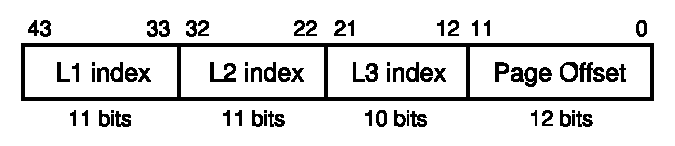
\includegraphics[width=0.45\textwidth]{./gfx/vaddr}
	    \caption{Composición de las direcciones virtuales (4KB).}
	    \label{fig::vaddr4k}
	    \end{figure}

	    Definiendo el overhead de traducción (PTO), como el cociente
	    entre (numerador) la cantidad de memoria fí­sica usada para
	    almacenar las tablas de paginación, y (denominador) la cantidad
	    de memoria fí­sica dedicada a páginas de código y datos de 
	    usuario, ¿cuál es el menor PTO posible en un esquema jerárquico
	    de tres niveles? ¿Cuál es el mayor valor del PTO? Suponer que
	    existe suficiente memoria fí­sica, como para que no haya swap de
	    páginas a disco; y usar PTEs de 64 bit. Además, a los efectos 
	    del cálculo, considerar que el contenido completo de la página
	    alocada es útil.

    \item	MIPS R10000 usa direcciones fí­sicas de 40 bit. La sección de
	    traducción de la TLB contiene el número de página fí­sica 
	    (\verb|PFN|), un bit \verb|V| para indicar si la entrada es
	    válida, un bit \verb|D| (dirty) para indicar que la página
	    necesita ser procesada debido a que fue modificada, y tres bits
	    de estado.

	    ¿Cuál es el tamaño mí­nimo de la PTE, suponiendo páginas de 4KB?

    \item	MIPS/Linux almacena cada PTE en una palabra de 64 bit. Usando
	    la respuesta a la última pregunta, ¿cuántos bits serán
	    desperdiciados?

    \item	\label{asdf}

	    El siguiente comentario, extraí­do de una versión de Linux/MIPS,
	    describe la jerarquía de tres niveles:

	    \begin{verbatim}
		/*
		  * Each address space has 2 4K pages as its page directory, giving
		  * 1024 8 byte pointers to pmd tables. Each pmd table is a pair of
		  * 4K pages, giving 1024 8 byte pointers to page tables. Each (3rd
		  * level) page table is a single 4K page, giving 512 8 byte ptes.
		  */
	    \end{verbatim}

	    Completar el cuadro \ref{tbl::answer}, suponiendo páginas de
	    4KB.

	    \begin{table}
	    \begin{center}
	    \begin{tabular}{|l|l|}
	    \hline
	    \textbf{Index} & \textbf{Longitud en bits}\\ \hline
	    Top-level      & \,                       \\ \hline
	    $2^{nd}$-level & \,                       \\ \hline
	    $3^{rd}$-level & \,                       \\ \hline
	    \end{tabular}
	    \caption{ver ejercicio \ref{asdf}.}
	    \label{tbl::answer}
	    \end{center}
	    \end{table}

    \item	Durante el diseño de un cache 4-way set associative, Raúl R.
	    nota que el cache sufrirá un problema de aliasing homónimo:
	    tal problema sucede cuando dos procesos usan la misma dirección
	    virtual para acceder a lugares fí­sicos distintos.

	    Raúl entonces consulta con el licenciado Varela, quien sugiere
	    agregar un campo PID (process id) al tag virtual. ¿Solucionará
	    esto el problema de aliasing?

	    Otro problema que surge al usar caches virtualmente indexados,
	    y virtualmente taggeados, es la aparición de sinónimos: los
	    mismos aparecen cuando direcciones virtuales distintas refieren
	    al mismo lugar fí­sico. ¿Solucionará este problema la idea del
	    licenciado?

	    Raúl piensa que otra forma de solucionar estos problemas, será
	    usando un cache direct mapped, en vez de set associative. 
	    ¿Tiene razón?
    \end{enumerate}


\subsection{}

  Considerar una máquina con direcciones virtuales de 64 bits y páginas de 4KB.
  Cuenta con una tabla de páginas jerárquica de tres niveles, donde los
  í­ndices L1, L2 y L3 son de 12 bits cada uno. Los bits más significativos
  no se utilizan. Ver cuadro \ref{tbl:vm_addr_fmt}.

  \begin{table}[h]
  \begin{center}
  \begin{tabular}{|c|c|c|c|c|}
  \hline
  unused & L1 index & L2 index & L3 index & page offset \\
  \hline
  \multicolumn{3}{l}{63} & \multicolumn{2}{r}{0} \\
  \end{tabular}
  \caption{Formato de las direcciones virtuales}
  \label{tbl:vm_addr_fmt}
  \end{center}
  \end{table}

  \begin{enumerate}
  \item ¿Cuántas entradas hay en la tabla de páginas del nivel 1?
  \item ¿Cuál es el tamaño de la parte implementada del espacio de direcciones virtuales?
  \item La figura \ref{fig:vm_mem_dump} muestra fragmentos del contenido de la
	tabla de páginas jerárquica de tres niveles (la columna a la izquierda
	corresponde a las direcciones fí­sicas de cada entrada en memoria).

	Las PTEs en las tablas de nivel 1 y 2 contienen la dirección fí­sica
	(PA) a o el número de bloque de disco (DBN) de la tabla del
	siguiente nivel.

	Las PTEs de la tabla de nivel 3 contiene el número de página fí­sica
	(PPN) o el número de bloque de disco (DBN) de la página accedida.
	Las direcciones fí­sicas son de 28 bits.
	
	El tamaño de las PTEs es de 4 bytes, y la dirección base (valor de 
	root pointer) de la tabla actual es 0x0004000. Las direcciones más
	bajas corresponden a los í­ndices más bajos de las tablas de páginas.
	Sólo se muestran las páginas válidas. La columna ``R'' indica el bit
	de página ``residente'' (o presente en memoria).
  
	Para cada dirección virtual dada a continuación, indicar la
	respuesta correcta y llenar el espacio en blanco si corresponde:
  
	\begin{enumerate}
	\item Recorrido de las tablas de paginación para la $VA = 0x0000004010110804$
	      \begin{enumerate}
	      \item Page table entry invalid exception
	      \item Page fault on page table entry
	      \item Page fault, disk block number \underline{$\qquad\qquad\qquad$}
	      \item Redisent, physical address \underline{$\qquad\qquad\qquad$}
	      \end{enumerate}
	\item Recorrido de las tablas de paginación para la $VA = 0x00000001113B0110$
	      \begin{enumerate}
	      \item Page table entry invalid exception
	      \item Page fault on page table entry
	      \item Page fault, disk block number \underline{$\qquad\qquad\qquad$}
	      \item Redisent, physical address \underline{$\qquad\qquad\qquad$}
	      \end{enumerate}
	\item Recorrido de las tablas de paginación para la $VA = 0x0000001101002CD0$
	      \begin{enumerate}
	      \item Page table entry invalid exception
	      \item Page fault on page table entry
	      \item Page fault, disk block number \underline{$\qquad\qquad\qquad$}
	      \item Redisent, physical address \underline{$\qquad\qquad\qquad$}
	      \end{enumerate}
	\end{enumerate}
\begin{figure}[h]
	\centering
	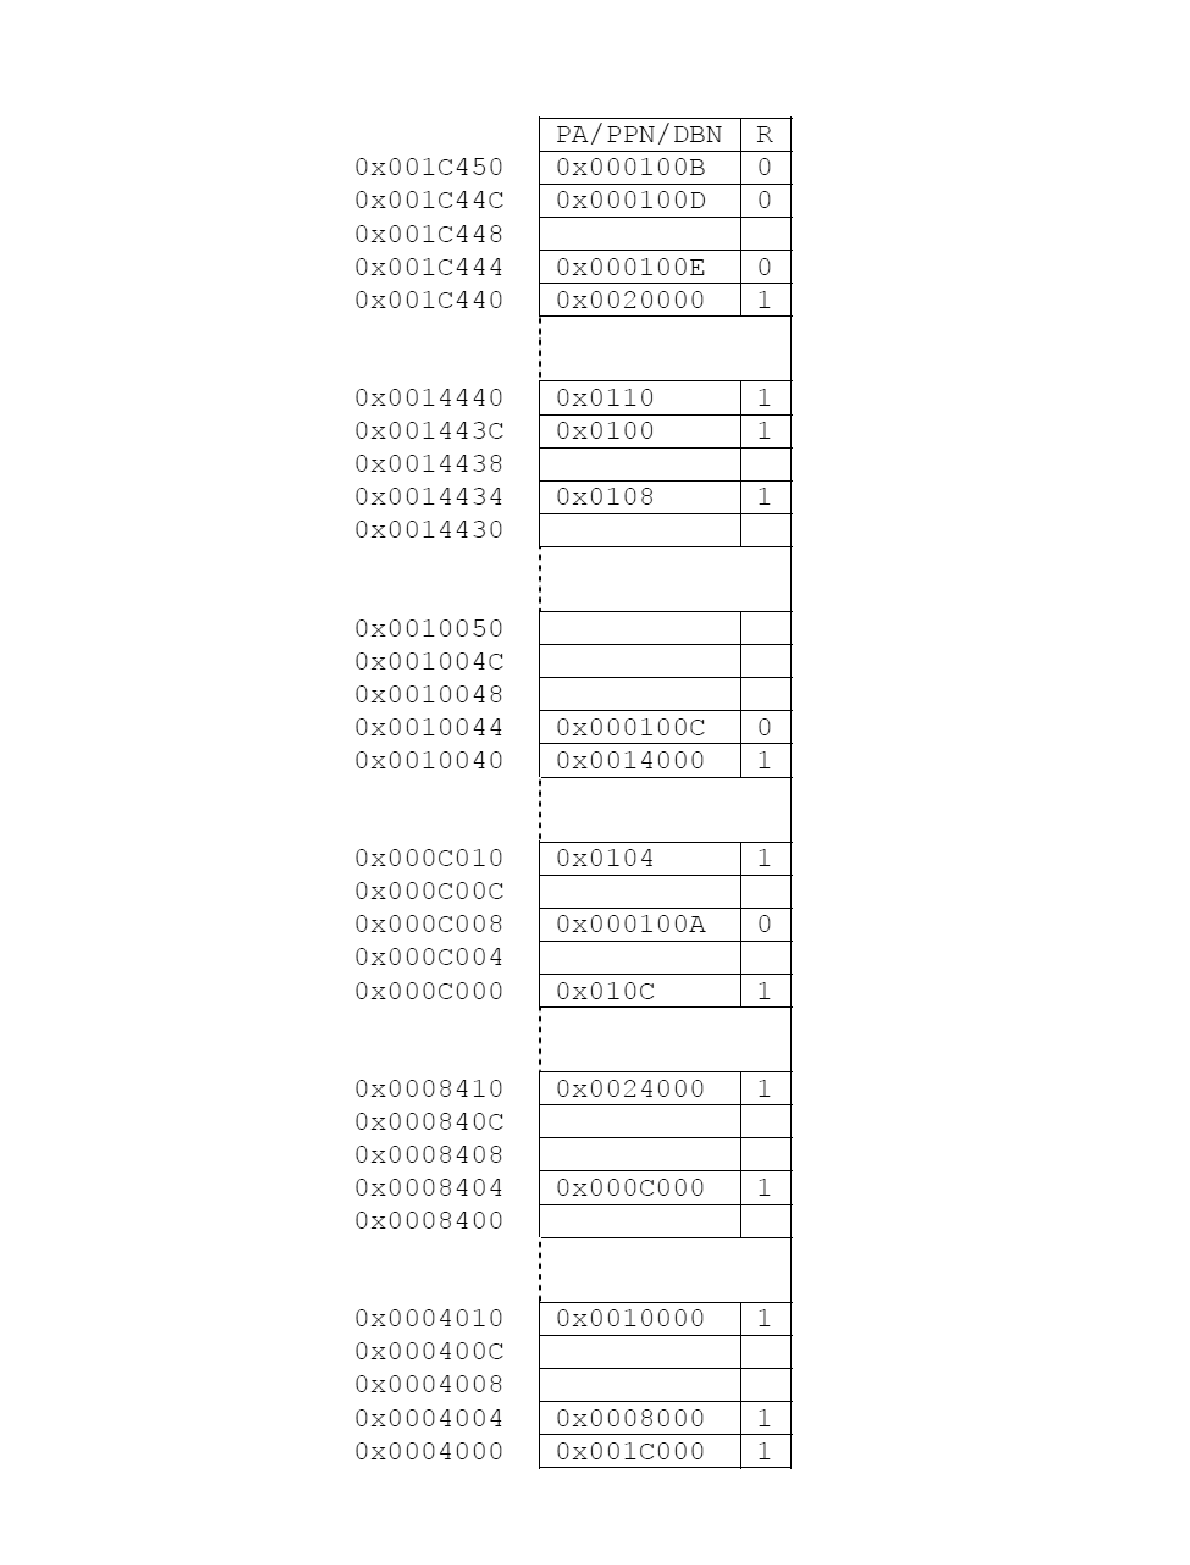
\includegraphics[width=0.7\textwidth]{./gfx/vm_mem_dump}
	\caption{Volcado de memoria en la región de la tabla de páginas}
	\label{fig:vm_mem_dump}
	\end{figure}

	\item La máquina descripta cuenta con un caché
	      único L1, el cual es accedido en paralelo con una TLB fully-associative
	      de 64 entradas. El caché es Direct Mapped, de 16KB, bloques de 4 words,
	      virtually-indexed y physically-tagged. El tamaño del word es de 4 bytes.
	      
	      \begin{enumerate}
	      \item ¿Cuáles de los 64 bits de la dirección virtual son traducidos 
		    por la TLB?
		    \underline{$\qquad\qquad$} : \underline{$\qquad\qquad$}
	      	      
	      \item ¿Cuáles de los 64 bits de la dirección virtual se utilizan para
		    indexar dentro del cache L1?
		    \underline{$\qquad\qquad$} : \underline{$\qquad\qquad$}
	      
	      \item ¿Cuáles de los 28 bits de la dirección fí­sica forman el cache tag?
		    \underline{$\qquad\qquad$} : \underline{$\qquad\qquad$}
	      	      
	      \end{enumerate}
	
	\item En este sistema se previene \emph{aliasing} de la
	      siguiente manera: si dos direcciones virtuales mapean a la misma
	      dirección fí­sica, se requiere que el sistema operativo haga que los
	      page offsets de las direcciones virtuales coincidan. ¿Esto funciona?
	      (justifique, de lo contrario la respuesta se considera automáticamente
	      incorrecta)
	
	\end{enumerate}

\subsection{}
    Sea un sistema de memoria virtual que permite alojar páginas de
    4KB y 4MB. El sistema usa 44 bits efectivos para describir direcciones
    virtuales, y 40 para direcciones físicas. Las páginas de 4KB son
    organizadas usando una tabla jerárquica de tres niveles; y las de 4MB
    se organizan usando los dos primeros niveles de la misma tabla.

    Para distinguir entre ambos casos, las L2 PTEs contienen información
    que indican si el puntero apunta a una tabla L3, o a una página de 4MB.
    Todas las PTEs son de 8 bytes. Ver figura \ref{fig::hier}.

    \begin{figure}[!ht]
    \centering
    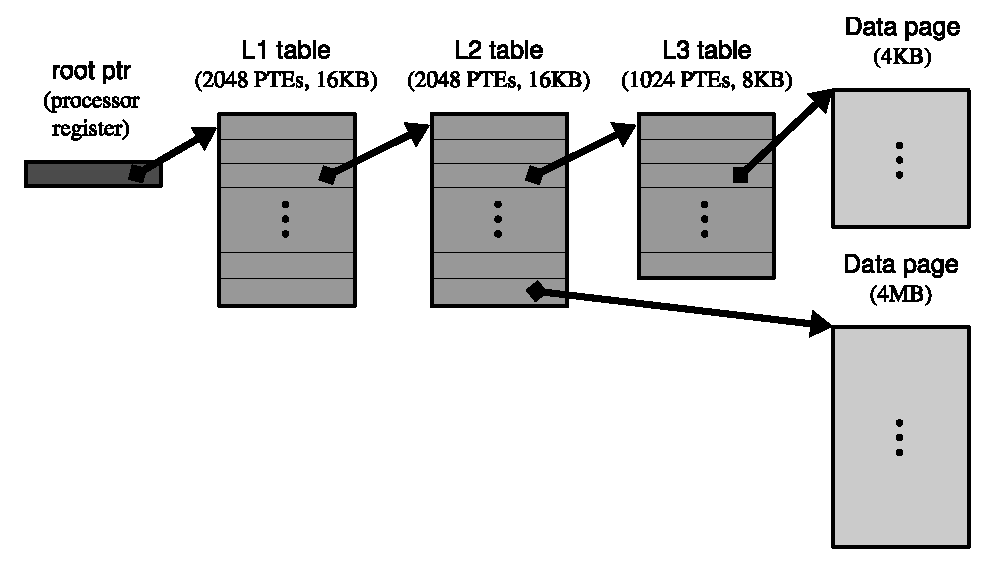
\includegraphics[width=0.6\textwidth]{./gfx/ptes.eps}
    \caption{jerarquía de traducción de direcciones.}
    \label{fig::hier}
    \end{figure}

    El procesador dispone de un TLB de datos con 64 entradas, y cada 
    entrada puede mapearse a cualquiera de los dos tipos de página, 4KB ó
    4MB. Al ocurrir un TLB miss, las tablas de traducción son recorridas
    por hardware, a fin de recargar el TLB. La política de reemplazo es
    FIFO.

    En este ejercicio, evaluaremos la ejecución y utilización de memoria
    del siguiente programa; el mismo es usado para sumar dos arreglos, y
    almacenar el resultado en un tercero:

    \begin{small}
    \begin{verbatim}
	uint8_t A[1048576]; /* 1MB array */
	uint8_t B[1048576]; /* 1MB array */
	uint8_t C[1048576]; /* 1MB array */
	for(int i = 0; i < 1048576; ++i)
		C[i] = A[i] + B[i];
    \end{verbatim}
    \end{small}

    Suponemos, además, que los arreglos \verb|A|, \verb|B|, y \verb|C| 
    están ubicados en una región contigua de memoria física. 
    Consideraremos, además, dos mapeos posibles:

    \begin{itemize}
    \item	4KB: los arreglos son mapeados usando 768 páginas de 4KB (es
	    decir, cada arreglo usa 256 páginas);

    \item	4MB: los arreglos son mapeados usando una única página.
    \end{itemize}

    En las preguntas que siguen, suponer que el programa es el único 
    proceso en el sistema, e ignorar cualquier overhead asociado a la
    ejecución de las instrucciones, o con el sistema operativo. Suponer
    que los arreglos están alineados de tal forma, que minimizan el
    número de PTEs involucradas.

    \begin{enumerate}
    \item	El particionado de la dirección virtual, en el caso de 4KB,
	    es: 11 bits (L1 index), 11 bits (L2 index), 10 bits (L3 index),
	    12 bits (page offset). Ver figura \ref{fig::vaddr4k}.

	    \begin{figure}[!ht]
	    \centering
	    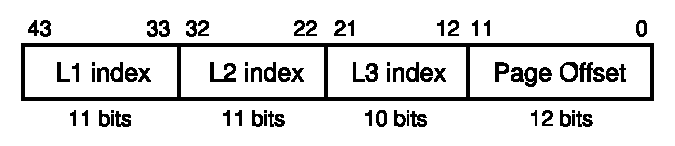
\includegraphics[width=0.45\textwidth]{./gfx/vaddr.eps}
	    \caption{composición de las direcciones virtuales (4KB).}
	    \label{fig::vaddr4k}
	    \end{figure}

	    Mostrar, en forma similar, cómo sería el particionado de una
	    dirección virtual que mapee a una página de 4MB. Incluir el
	    nombre y longitud en bits de todos los campos involucrados.
    
    \item	Definimos el overhead de traducción (PTO), como el cociente 
	    entre (numerador) la cantidad de memoria física usada para
	    almacenar las tablas de paginación, y (denominador) la cantidad
	    de memoria física dedicada a páginas de datos.

	    Para el programa dado anteriormente, ?`cuál es el $PTO_{4KB}$?
	    ?`cuál es el $PTO_{4MB}$?

    \item	Definimos el overhead de fragmentación (PFO), como el cociente
	    entre (numerador) la cantidad de memoria física dedicada a
	    páginas de datos, pero que nunca es accedida; y (denominador)
	    cantidad de memoria física alocada a páginas de datos, 
	    accedida.

	    Para el programa visto, ?`cuánto valen $PFO_{4KB}$ y
	    $PFO_{4MB}$?

    \item	Consideremos ahora la ejecución del programa, suponiendo que
	    la TLB está inicialmente vacía. Para cada uno de los casos
	    (i.e. 4KB y 4MB), ?`cuántos TLB misses ocurren, y cuántos
	    accesos a memoria (PTEs) son necesarios para recargar la TLB?

    \item	?`Cuál de los siguientes números es el mejor candidato para
	    estimar (orden de magnitud) el speedup? 
	    $SU = \left\{1.01; 10; 1000; 1000000\right\}$. Elegir uno, 
	    explicando brevemente tu respuesta. Tomar el caso de 4KB como
	    referencia.
    \end{enumerate}




% 
% \begin{thebibliography}{9}
% 
%     \bibitem{caaqa}
%     David Patterson, John Hennessy, \textit{Computer Architecture a Quantitative Approach}, Elsevier, 3rd edition. ISBN: 1-55860-596-7. May 2002.  
%   
%     \bibitem{coadhsi}
% 
%     David Patterson, John Hennessy, \textit{Computer Organization and Design, the Hardware/Software Interface},  Elsevier, 3rd edition. ISBN: 1-55860-604-1. Aug. 2004. 
%     
%     \bibitem{vmp1}
% 
%     B.L. Jacob and T.N. Mudge, \textit{Virtual Memory: Issues of Implementation}, Computer, Vol. 31, No. 6, June 1998, pp. 33-43.
% 
%     \bibitem{vmp2}
% 
%     B.L. Jacob and T.N. Mudge, \textit{Virtual Memory in Contemporary Microprocessors}, IEEE Micro, Aug. 1998.
%     
%     \bibitem{mafstocm}
% 
%     Jean-Loup Baer, \textit{Microprocessor Architecture. From Simple Pipelines to Chip Multiprocessors}, Cambridge University Press. ISBN-13 978-0-521-76992-1. 2010
% 
% 
%     \bibitem{mcch}
%     
%     Rajeev Balasubramonian and Norman P. Jouppi and Naveen Muralimanohar, \textit{Multi-Core Cache Hierarchies}, Morgan and Claypool Publishers, 2011.
%     
%     \bibitem{abi}
%     
%     System V Application Binary Interface, MIPS RISC Processor, 3rd Edition, The Santa Cruz Operation, February 1996 (http://www.sco.com/developers/devspecs/mipsabi.pdf).
% \end{thebibliography}
\end{document}
